\chapter{Introduction and Literature Review}

\begin{quote}
Choreographic programming is a language paradigm for writing concurrent software systems of various kinds.
It's comparatively young; while some of the ideas have existed informally as far back as the 1970s,
choreographic programming as it's understood today was first formalized in~\shortcite{montesi-carbone-dfbd}.
In this chapter we describe the central concepts of choreographic programming,
its advantages and disadvantages,
and past and ongoing work to push the boundaries of the kinds of systems it can implement.
\end{quote}

\section{Introduction}

Choreographic programming (CP)
is a paradigm for implementing distributed systems in which the programmer writes one unified program, called a choreography,
that describes how the participants of the system interact
from a third-person-omniscient perspective.~\shortcite{montesi-carbone-dfbd,montesi-dissertation,montesi_book}
A choreography can be translated into to a collection of executable programs for use in the real world, one for each participant;
this process is called endpoint projection (EPP).
The CP approach has benefits both for understandability of distributed system implementations,
and for strong static guarantees about the deadlock-freedom of the resulting executable code~\cite{montesi-carbone-dfbd}.

\subsection{An illustrative example}

Consider the three programs in \Cref{fig:kvspiecewise},
which are intended to run concurrently and pass messages back and forth between each other.
The overall effect is an elementary process in which the client makes a \inlinecode{Get} or \inlinecode{Put} request to
a server (with a backup) that manages a key-value-store (KVS).
Even this simplified example takes a moment for a reader to make sense of;
one must read the three programs, infer the correspondence between messages sent and received by the three parties,
and judge for oneself if the communication protocol implemented is sensical.
One might even judge that this simple protocol has a bug:
if the request is a \inlinecode{Get}, the backup server will hang indefinitely!

\begin{figure}[tbhp]\caption{A Simple Concurrent Protocol: a key-value store with a backup server}
  \begin{mdframed}
  \begin{tabular}{c}
  \begin{minipage}{12.5cm}
    \inputminted[xleftmargin=10pt,linenos,fontsize=\scriptsize]{haskell}{figures/kvs_piecewise_client.hs.txt}
  \end{minipage} \\\\
  \begin{minipage}{12.5cm}
	  \textbf{(a)} The function to be called by the client process.
	  They pass in their \inlinecode{Request} object and send it to the server.
	  Then they receive a response from the server and return it.
  \end{minipage}\\\\
  \hline\\
  \begin{minipage}{12.5cm}
    \inputminted[xleftmargin=10pt,linenos,fontsize=\scriptsize]{haskell}{figures/kvs_piecewise_server.hs.txt}
  \end{minipage} \\\\
  \begin{minipage}{12.5cm}
  The function to be called by the primary server.
	  They pass in a reference to their mutable state, and receive a message of type \inlinecode{Request} from the client.
	  In the case of a \inlinecode{Put} request, they forward it to the backup server and check for the backup's acknowledgement.
	  In either case, they process the request against their own mutable state and send the response back to the client.
  \end{minipage}\\\\
  \hline\\
  \begin{minipage}{12.5cm}
    \inputminted[xleftmargin=10pt,linenos,fontsize=\scriptsize]{haskell}{figures/kvs_piecewise_backup.hs.txt}
  \end{minipage} \\\\
  \begin{minipage}{12.5cm}
  The function to be called by the backup server.
	  They pass in a reference to their mutable state, and receive a \inlinecode{Put} message from the primary server.
	  They process it against their mutable state and send back an acknowledgement message to indicate their success.
  \end{minipage}
  \end{tabular}
  \label{fig:kvspiecewise}
  \end{mdframed}
\end{figure}

In \Cref{sec:background} we will mention some intermediate frameworks that have historically been used to facilitate
writing large and complicated concurrent protocols,
but here we jump ahead to choreographic programming (CP).
\Cref{fig:kvspseudo} shows the same protocol as \Cref{fig:kvspiecewise}, but implemented as a choreography.
In this form there is no cognitive overhead for matching \inlinecode{send} and \inlinecode{recv} operations,
because matching pairs of them are combined into monolithic \inlinecode{comm} operations.
The entire protocol can be read at once in a sensical order.
(The order in which operations are presented in a choreography is not necessarily the order in which they will happen;
the participants are not guaranteed to all start at the same physical time, or to operate at the same speeds.)
Re-writing the example KVS system as a choreography does not immediately solve the issue
of what the backup server should do in the event of a \inlinecode{Get} request,
but it makes the problem detectable by static analysis.
In fact, the choreography in \Cref{fig:kvspseudo} cannot compile in any real CP system
because \inlinecode{"backup"}'s behavior is ambiguous.
\Cref{fig:kvsenclave} shows two variations of how to realize the KVS behavior in Haskell using our \MultiChor library.

\begin{figure}[tbhp]\caption{A Simple Choreography: a key-value store with a backup server}
  \begin{mdframed}
  \begin{tabular}{c}
  \begin{minipage}{12.5cm}
    \inputminted[xleftmargin=10pt,linenos,fontsize=\scriptsize]{haskell}{figures/kvs_pseudo.hs.txt}
  \end{minipage} \\\\
  \begin{minipage}{12.5cm}
	  A pseudo-code choreographic implementation of the protocol from \Cref{fig:kvspiecewise}.
  \end{minipage}
  \end{tabular}
  \label{fig:kvspseudo}
  \end{mdframed}
\end{figure}


\begin{figure}[tbhp]\caption{A Real Choreography: a key-value store writing using \MultiChor}
  \begin{mdframed}
  \begin{tabular}{c c}
  \begin{minipage}{8.75cm}
    \inputminted[xleftmargin=10pt,linenos,fontsize=\scriptsize]{haskell}{figures/kvsenclave_a.hs.txt}
  \end{minipage}
  &
  \begin{minipage}{3.75cm}
    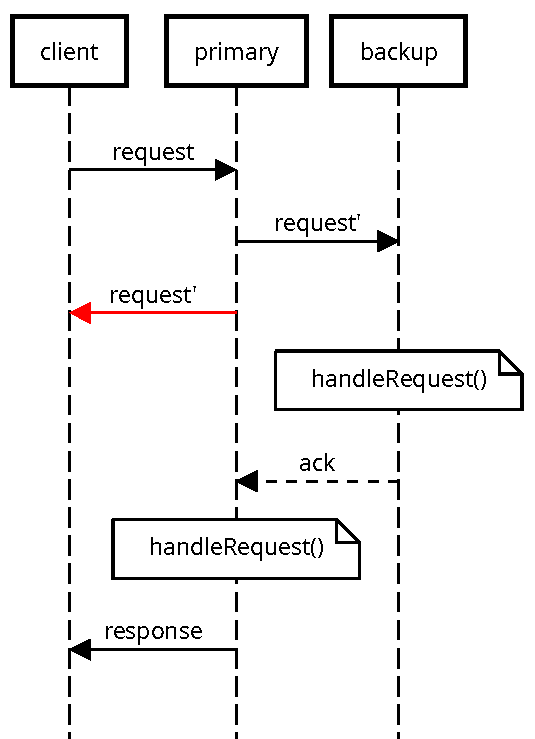
\includegraphics[width=4cm]{figures/seq2.pdf}
  \end{minipage} \\\\
  \multicolumn{2}{c}{\begin{minipage}{12.5cm}
  A key-value store with a backup server, written in \MultiChor.
           The backup server sends an acknowledgement message \textsf{ack} to the primary server
           if and only if \inlinecode{request} is a \inlinecode{Put}.
           The \inlinecode{broadcast} operator (line 19) ensures KoC
           so that the primary and backup servers are guaranteed to use the same case of \inlinecode{handleBackup},
           but it results in redundant communication (shown in red in the sequence diagram).
  \end{minipage}}\\\\
  \hline\\
  \begin{minipage}{8.75cm}
    \inputminted[xleftmargin=10pt,linenos,fontsize=\scriptsize]{haskell}{figures/kvsenclave_b.hs.txt}
  \end{minipage}
  &
  \begin{minipage}{3.75cm}
     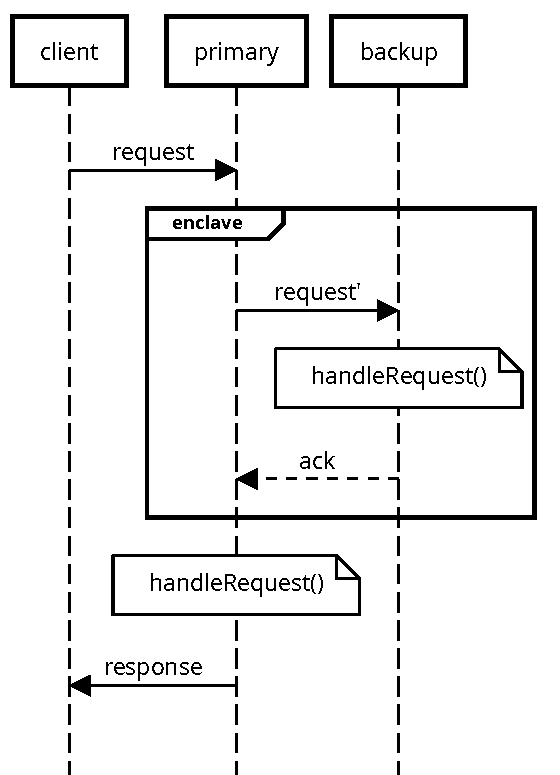
\includegraphics[width=4cm]{figures/seq3.pdf}
  \end{minipage} \\\\
  \multicolumn{2}{c}{\begin{minipage}{12.5cm}
  In this variation, the \inlinecode{enclave} operator eliminates the redundant communication.
           The enclaved sub-choreography is indicated by a box in the sequence diagram.
           On line~2, \inlinecode{@@ nobody} is \MultiChor idiom explained in \Cref{sec:membership}.
  \end{minipage}}
  \end{tabular}
  \label{fig:kvsenclave}
    %%\Description{In the top section, twenty four lines of Haskell code using the MultiChor library, with a UML sequence diagram of that program.
%%	The code defines a choreography called "kvs", and helper-functions "handleRequest" and "handleBackup".
%%	In the sequence diagram, first "client" sends "request" to "server",
%%	  then "server" sends "request-prime" to "client" and "backup",
%%	  then backup calls "handleRequest",
%%	  then backup may send "ack" to "server",
%%	  then server calls "handleRequest",
%%	  then server sends "response" to "client.
%%	The bottom sections shows changes to the code in the top section.
%%	In particular, the return type of "handleBackup" is changed to exclude "client".
%%	In the updated sequence diagram, the part of the protocol representing "handleBackup" is in a box named "enclave",
%%	  and the spurious transmission of "request-prime" from "server" to "client" is omitted.
%%	  }
  \end{mdframed}
\end{figure}


Here is a citation, \shortcite{li2021model}.

\subsection{Layout and Contributions}

The remainder of this chapter covers the history and theory of CP
and discusses some modern work relevant to the ongoing development of CP systems.
In particular, \Cref{sec:knowledge-of-choice} discusses the "Knowledge of Choice" problem,
a central difficulty in the design of CP systems,
and a number of strategies that have been used to solve it.

\Cref{sec:formalism} presents our first contribution:
a formal model of a CP system with two novel features:
\emph{multiply-located values} (MLVs)
and \emph{enclaves}.
These features combine to allow a compelling new strategy for KoC management.
In particular, all well-typed \HLSCentral choreographies are projectable and have cromulent KoC by construction.
In \Cref{sec:formalism-comparisons} we compare \HLSCentral to representative systems that use other KoC management strategies.

\Cref{sec:multichor} presents our implementation of the enclaves-\&-MLVs paradigm in Haskell.
The \MultiChor library is already available on Hackage, Haskell's main package management system.
\MultiChor directly implements the main concepts of \HLSCentral as a monadic eDSL in Haskell,
and combines Haskell's Hindley–Milner-based type system with a proof-witness system
to capture the requisite notion of a well-typed choreography.
Because \MultiChor is fully embedded in and interoperable with Haskell,
functional-programming patterns can be applied to the choreographic setting without further theoretical or infrastructural work.
The most important example of this, which we call "census polymorphism" is the ability to write choreographies
that are parametric over their set of participants.
We discuss census polymorphism in greater detail in \Cref{sec:census-poly}.
\Cref{sec:future-implementation} reviews some promising future, both theoretical and at the engineering level,
that could improve \MultiChor's utility.



\section{Background}
\label{sec:background}
In this section, we give a brief overview of choreographic programming (CP).
For a comprehensive introduction to the topic, we refer the reader to~\cite{montesi_book}.

Choreographic programming is a paradigm that expresses a distributed system
as a single, global program describing the behavior and interactions of all parties.
The global view of the distributed system enables easier reasoning about the system's behavior;
for example choreographic languages can ensure \emph{deadlock freedom}~\cite{montesi-carbone-dfbd}
and choreographies can be composed modularly like normal single-threaded protocols.



\subsection{Knowledge of Choice}
\label{sec:knowledge-of-choice}

Choreographies with conditionals
(\inlinecode{if}-expressions or anything that could be used for conditional control-flow)
introduce
a challenge for endpoint projection:
\emph{some parties might not know which branch to take!}
This challenge is referred to as the \emph{knowledge of choice}  (KoC)~\cite{castagna-knowledge-of-choice} problem.
All choreographic programming languages include a strategy for KoC
that ensures that relevant parties have enough information to play their part in the program.

\subsection{Endpoint Projection}
\label{sec:endpoint-projection}
Maybe this goes before KoC; I haven't decided.

\subsection{Additional Literature}
\label{sec:modern-work}

Review recent work on CP systems, including other systems that use MLVs.


\bibliographystyle{chicago}
\bibliography{refs}
